The method described here was proposed in \cite{SVIclassification}. We could also apply the svi method to the classification problem. In order to do so, we will first rederive the ELBO from (\ref{L3}).

We will use the augmented model for the data.
$$p(y, f, u) = p(y | f) p(f | u) p(u).$$
\begin{figure}[!h]
	\centering
	\subfloat{
		\scalebox{0.7}{
			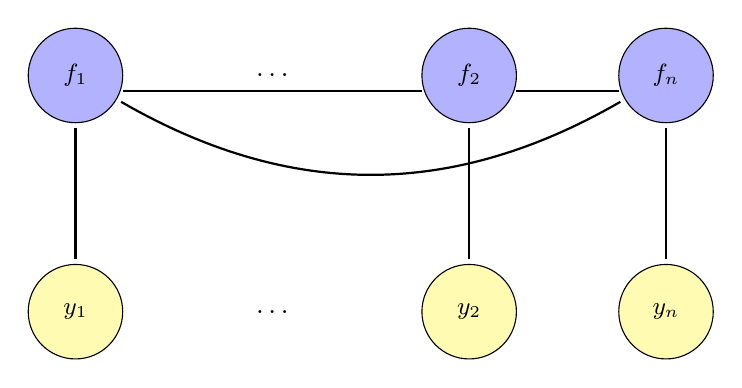
\begin{tikzpicture}
	\tikzstyle{x_i} = [circle, draw, fill=green!50, minimum size=1.2cm, text width=0.8cm, align=center, font=\large]
	\tikzstyle{f_i} = [circle, draw, fill=blue!30, minimum size=1.2cm, inner sep=2pt, outer sep=2pt, font=\small, align=center]
	\tikzstyle{y_i} = [circle, draw, fill=yellow!30, minimum size=1.2cm, inner sep=2pt, outer sep=2pt, font=\small, align=center]
	\tikzstyle{edge_label} = [font=\small, label={[label distance = -4pt]90:$\text$}]
	\tikzstyle{edge} = [thick, >=stealth]
	\tikzstyle{biedge} = [thick, >=stealth]
	\def\step{-3}
	\def\layerpos{3}

	\foreach \name/\x in {f_1/-2.5, f_2/2.5, f_n/5} 
	  	\node[f_i] (\name) at (\x, \layerpos) {$\name$};

	\draw[biedge] (f_1)++(0.6,-0.2) -- ++(3.8,0); %(f_2);
	\draw[biedge] (f_2)++(0.6,-0.2) -- +(1.3,0);% ++ (f_n);
	\draw [biedge] (f_1) to [out=-30,in=-150] (f_n);
	\node (other^2) at (0, \layerpos) {$\ldots$};

	%observables
	\pgfmathsetmacro{\layerpos}{\layerpos + \step}

	\foreach \name/\x in {y_1/-2.5, y_2/2.5, y_n/5} 
	  	\node[y_i] (\name) at (\x, \layerpos) {$\name$};

	\node (other^3) at (0, \layerpos) {$\ldots$};
	\foreach \from/\to in {f_1/y_1, f_2/y_2, f_n/y_n}
		\draw[edge] (\from) -- (\to);
\end{tikzpicture}
		}
	}
	\hspace{1cm}
	\subfloat{
		\scalebox{0.7}{
			\input{../pictures/inducing_input_gp_gm.tikz}
		}
	}
	\caption{Graphical models for standard and inducing-point gaussian process classification}
\end{figure}

Applying the standard variational lower bound to this model, we obtain
$$\log p(y) \ge \E_{q(u, f)} \log \frac {p(y, u, f)}{q(u, f)} = \E_{q(u, f)}\log p(y | f) - \KL{q(u, f)} {p(u, f)}.$$
Our model implies $\E_{q(u, f)} \log p(y | f) = \E_{q(f)} \log p(y | f)$, where $q(f)$ is the marginal of $q(u, f)$.

We will consider the variational distributions of the following form:
$$q(u, f) = p(f | u) q(u),$$
where $q(u) \sim \N(u|\mu, \Sigma)$. This implies $q(f)$
$$q(f) = \int p(u | f) q(u) du = 
\N(f| K_{nm} K_{mm}^{-1} \mu, K_{nn} + K_{nm} K_{mm}^{-1}(\Sigma - K_{mm}) K_{mm}^{-1} K_{mn}).$$

Now, consider the KL-divergence in the lower bound we've devised.
$$\KL{q(u, f)} {p(u, f)} = \KL{q(u) p(f|u)} {p(u) p(f|u)} = \KL{q(u)} {p(u)}.$$

Finally, the lower bound is
\begin{equation}\label{sviELBO}
	\log p(y) \ge \E_{q(f)} \log p(y | f) - \KL{q(u)} {p(u)} = $$ $$ = \sum_{i = 1}^{n} \E_{q(f_i)} \log p(y_i | f_i) - \KL{q(u)} {p(u)},
\end{equation}
where 
$$q(f_i) = \N(f_i | k_i^T K_{mm}^{-1} \mu, K_{ii} + k_i^T K_{mm}^{-1} (\Sigma - K_{mm}) K_{mm}^{-1} k_{i}) = \N(f_i | m_i, S_i^2)$$
Note, that this lower bound is exactly the lower bound from (\ref{L3}), but now, we've derived it in a more general setting.

% Note, that 
% $$\E_{q(f_i)} \log p(y_i|f_i) = \E_{\N(f_i| m_i, S_i)} \log p(y_i|f_i) = \E_{\N(t | 0, 1)} \log p(y_i | (t \sqrt{S_i} + m_i))$$

Substituting the distributions $q$ and $p$ back into the (\ref{sviELBO}) we obtain

% $$\log p(y) \ge \sum_{i=1}^n \E_{\N(t | 0, 1)} \log p(y_i | t \sqrt{S_i} + m_i) -$$    
$$\log p(y) \ge \sum_{i=1}^n \E_{\N(f_i | m_i, S_i^2)} \log p(y_i | f_i) -$$
\begin{equation}\label{explicit_svi_elbo}
	-\frac 1 2 \left (\log \frac {|K_{mm}|} {|\Sigma|} - m + \tr(K_{mm}^{-1} \Sigma) + \mu^T K_{mm}^{-1} \mu \right) = L_3(\mu, \Sigma, \theta).
\end{equation}

Now we can maximize this lower bound with respect to variational parameters $\mu$, $\Sigma$ and covariance hyper-parameters $\theta$.

Let's find the derivatives of (\ref{explicit_svi_elbo}).

% $$\derivative{L_3}{\mu} = \sum_{i=1}^n \derivative{}{\mu} \E_{\N(t | 0, 1)} \log p(y_i | t \sqrt{S_i} + m_i) + K_{mm}^{-1} \mu = $$
$$\derivative{L_3}{\mu} = \sum_{i=1}^n \derivative{}{\mu} \left(\E_{\N(f_i | m_i, S_i^2)} \log p(y_i | f_i)\right) - K_{mm}^{-1} \mu = $$
$$ = \sum_{i=1}^n \derivative{}{m_i} \left(\E_{\N(f_i | m_i, S_i^2)} \log p(y_i | f_i)\right) \derivative{m_i}{\mu} - K_{mm}^{-1} \mu,$$
$$ = \sum_{i=1}^n \E_{\N(f_i | m_i, S_i^2)}\left[ \derivative{}{f_i} \log p(y_i | f_i)\right] \derivative{m_i}{\mu} - K_{mm}^{-1} \mu,$$

$$\derivative{L_3}{L_{\Sigma}} = \sum_{i=1}^n \derivative{}{S_i^2}\left( \E_{\N(f_i | m_i, S_i^2)} \log p(y_i | f_i)\right) \derivative{S_i^2}{L_{\Sigma}} + \hat L - K_{mm}^{-1} L_{\Sigma} = $$
$$= \frac 1 2 \sum_{i=1}^n \E_{\N(f_i | m_i, S_i^2)}\left[ \derivative{^2}{f_i^2} \log p(y_i | f_i)\right] \derivative {S_i^2}{L_{\Sigma}} + \hat L - K_{mm}^{-1} L_{\Sigma},$$
where
$$\hat L = 
\left(
\begin{array}{cccc}
\frac 1 {(L_{\Sigma})_{11}} & 0 & \ldots & 0\\
0 & \frac 1 {(L_{\Sigma})_{22}} & \ldots & 0\\
\ldots & \ldots & \ldots & \ldots\\
0 & 0 & \ldots & \frac 1 {(L_{\Sigma})_{mm}} \\
\end{array}   
\right) $$


$$\derivative{L_3}{\theta} = \derivative{}{\theta} \left(\sum_{i=1}^n \E_{\N(t | m_i, S_i^2)}  \log p(y_i | f_i)\right) -$$
$$- \frac 1 2 \tr\left(K_{mm}^{-1} \frac{\partial K_{mm}}{\partial \theta}\right) + \frac 1 2 \tr\left(\Sigma K_{mm}^{-1} \frac{\partial K_{mm}}{\partial \theta} K_{mm}^{-1} \right)+ \frac 1 2 \mu^T K_{mm}^{-1} \frac{\partial K_{mm}}{\partial \theta} K_{mm}^{-1}\mu.$$

Note that
$$\derivative{}{\theta} \left(\E_{\N(f_i | m_i, S_i^2)} \log p(y_i | f_i)\right) = \derivative{}{m_i}\left(\E_{\N(t | m_i, S_i^2)}  \log p(y_i | f_i) \right)\derivative{m_i}{\theta} + \derivative{}{S_i^2}\left(\E_{\N(f_i | m_i, S_i^2)}  \log p(y_i | f_i) \right)\derivative{S_i^2}{\theta} = $$
$$ = \E_{\N(f_i | m_i, S_i^2)} \left[\derivative{}{f_i} \log p(y_i | f_i) \right] \derivative{m_i}{\theta} + \frac 1 2 \E_{\N(f_i | m_i, S_i^2)} \left[\derivative{^2}{f_i^2} \log p(y_i | f_i) \right] \derivative{S_i^2}{\theta}$$

In order to compute the expectations in the derivatives, we can use the integral approximation techniques, and Gauss-Hermite quadrature in particular.

We will use logistic likelihood
$$\log p(y_i | f_i) =  - \log(1 + \exp( - y_i f_i)).$$

Then
$$\derivative{}{f_i} \log p(y_i | f_i) = \frac{y_i}{1 + \exp(y_i f_i)},$$
$$\derivative{^2}{f_i^2} \log p(y_i | f_i) = - \frac{y_i^2 \exp(y_i f_i)}{(1 + \exp(y_i f_i))^2}.$$

Now,
$$m_i = k_i^T K_{mm}^{-1} \mu,$$
$$\derivative{m_i}{\mu} = K_{mm}^{-1} k_i$$
$$\derivative{m_i}{\theta} = \derivative{k_i}{\theta}^T K_{mm}^{-1} \mu - k_i^T K_{mm}^{-1} \derivative{K_mm}{\theta} K_{mm}^{-1} \mu.$$
Finally, 
$$S_i^2 = K_{ii} + k_i^T K_{mm}^{-1} (L_\Sigma L_\Sigma^T - K_{mm}) K_{mm}^{-1} k_{i},$$
$$\derivative{S_i^2}{L_{\Sigma}} = 2 K_{mm}^{-1} k_i k_i^T K_{mm}^{-1} L_{\Sigma},$$
$$\derivative{S_i^2}{\theta} = \derivative{K_{ii}}{\theta} + 2 \derivative{k_i}{\theta}^T K_{mm}^{-1} (L_\Sigma L_\Sigma^T - K_{mm}) K_{mm}^{-1} k_{i}$$
$$ - 2 k_i^T K_{mm}^{-1} \derivative{K_{mm}}{\theta} K_{mm}^{-1} (L_\Sigma L_\Sigma^T - K_{mm}) K_{mm}^{-1} k_{i} - k_i^T K_{mm}^{-1} \derivative{K_{mm}}{\theta} K_{mm}^{-1} k_{i}.$$

The final formulas for the derevatives are
$$\derivative{L_3}{\mu} = \sum_{i=1}^n \E_{\N(f_i | m_i, S_i^2)}\left[\frac{y_i}{1 + \exp(y_i f_i)}\right] K_{mm}^{-1} k_i + K_{mm}^{-1} \mu,$$

$$\derivative{L_3}{L_{\Sigma}} = \sum_{i=1}^n \E_{\N(f_i | m_i, S_i^2)}\left[- \frac{y_i^2 \exp(y_i f_i)}{(1 + \exp(y_i f_i))^2} \right] K_{mm}^{-1} k_i k_i^T K_{mm}^{-1} L_{\Sigma} + \hat L - K_{mm}^{-1} L_{\Sigma},$$

$$\derivative{L_3}{\theta} = \sum_{i=1}^n \left[\E_{\N(f_i | m_i, S_i^2)} \left[\frac{y_i}{1 + \exp(y_i f_i)}\right] \left(\derivative{k_i}{\theta}^T K_{mm}^{-1} \mu - k_i^T K_{mm}^{-1} \derivative{K_mm}{\theta} K_{mm}^{-1} \mu \right)\right.$$
$$ + \frac 1 2 \E_{\N(f_i | m_i, S_i^2)} \left[- \frac{y_i^2 \exp(y_i f_i)}{(1 + \exp(y_i f_i))^2}\right] \left( \derivative{K_{ii}}{\theta} + 2 \derivative{k_i}{\theta}^T K_{mm}^{-1} (L_\Sigma L_\Sigma^T - K_{mm}) K_{mm}^{-1} k_{i} \right.$$
$$ \left.\left.- 2 k_i^T K_{mm}^{-1} \derivative{K_{mm}}{\theta} K_{mm}^{-1} (L_\Sigma L_\Sigma^T - K_{mm}) K_{mm}^{-1} k_{i} - k_i^T K_{mm}^{-1} \derivative{K_{mm}}{\theta} K_{mm}^{-1} k_{i} \right)\right]- $$
$$- \frac 1 2 \tr\left(K_{mm}^{-1} \frac{\partial K_{mm}}{\partial \theta}\right) + \frac 1 2 \tr\left(\Sigma K_{mm}^{-1} \frac{\partial K_{mm}}{\partial \theta} K_{mm}^{-1} \right)+ \frac 1 2 \mu^T K_{mm}^{-1} \frac{\partial K_{mm}}{\partial \theta} K_{mm}^{-1}\mu.$$




